\begin{center}
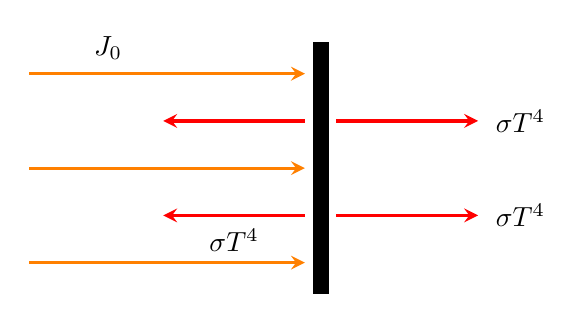
\begin{tikzpicture}[>=stealth]
 \fill[black] (0,-1.6) rectangle (0.2,1.6);
 \foreach \y in {-1.2,0,1.2} \draw[->, very thick, orange] (-3.6,\y) -- (-0.1,\y);
 \node[anchor=south] at (-2.6,1.25) {$J_0$};
 \foreach \y in {-0.6,0.6} \draw[->, very thick, red] (-0.1,\y) -- (-1.9,\y);
 \foreach \y in {-0.6,0.6} \draw[->, very thick, red] (0.3,\y) -- (2.1,\y);
 \node[anchor=west] at (2.2,0.6) {$\sigma T^4$};
 \node[anchor=west] at (2.2,-0.6) {$\sigma T^4$};
 \node[anchor=north] at (-1.0,-0.65) {$\sigma T^4$};
\end{tikzpicture}
\end{center}

Die schwarze Platte absorbiert die ganze einfallende Strahlung, pro Fläche $A$ die Leistung $J_0\,A$. Als schwarzer Körper ($\varepsilon = 1$) strahlt sie auf \emph{beiden} Seiten die Intensität $\sigma\,T^4$ ab, insgesamt $2\,\sigma\,T^4 A$. Im Gleichgewicht sind die beiden Leistungen gleich (Wärmeleitung an die Luft vernachlässigt):
\begin{align}
 J_0\,A &= 2\,\sigma\,T^4 A \\
 T &= \TpF \\
   &= \sqrt[4]{\frac{\Jo}{2\cdot\sig}} \\
   &= \Tp \approx \result{\TpP{0}{3}}
\end{align}
mit $\sigma$ aus FoTaBe (Umschlag hinten). Das entspricht $\vartheta = \tpP{0}{2}$.
